%%%%%%%%%%%%%%%%%%%%%%%%%%%%%%%%%%%%%%%%%%%%%%%%%%%%%%%%%%%%%%%%%%%%%%%%
\chapter{Related Work}
\label{sec:relatedWork}

In this chapter, I will discuss work which was relevant for the ChaCha plugin implementation in some way and was therefore reviewed by me during the work on this thesis.

%%%%%%%%%%%%%%%%%%%%%%%%%%%%%%%%%%%%%%%%%%%%%%%%%%%%%%%%%%%%%%%%%%%%%%%%
\section{Salsa20 Cipher Family}
\label{sec:salsaCipher}

The 256-bit stream cipher family Salsa20 is the cipher family on which the ChaCha cipher family is based on.

Salsa20/20, the 20 rounds variant, was developed by Prof. Daniel J. Bernstein in 2005 \cite{salsaspec} and submitted to eSTREAM, an european project to ``to promote the design of efficient and compact stream ciphers suitable for widespread adoption'' \cite{estream}.

It uses only add-rotate-XOR (ARX) operations for encryption which prevents timing attacks since they run in constant time on basically all platforms. Beside 256-bit keys, it also supports 128-bit keys. It internally uses a round function which transform a 512-bit state, consisting of the key, four 32-bit constants, a 64-bit initialization vector and a 64-bit counter, into a keystream block. Since for the next keystream block, only the counter is incremented in the initial state, Salsa20 shares the same implementation advantages as block ciphers in counter mode, in particular the ability to generate output blocks in any order and in parallel \cite{salsaspec}.

Prof. Bernstein later introduced other variants with 8 and 12 rounds, named Salsa20/8 and Salsa20/12, to let users decide between a faster, but less secure cipher. Other round variants like 9, 10 or 11 were not introduced because the difference in speed would be insignificant \cite{salsa812}. The ChaCha cipher family received the same round variants. 

There is also a variant of Salsa20 called XSalsa20 which supports 192-bit initialization vectors. Since its implementation varies quite a bit from the Salsa20/r variants and Prof. Bernstein introduced XSalsa20 as part of a new cipher family (based on Salsa20), this cipher is of no relevance for this thesis \cite{xsalsa20spec}. There is a XChaCha20 variant but it ``is currently not widely implemented outside the libsodium library [a software library for cryptography], due to the absence of formal specification'' \cite{xchacha20}.

The specification of Salsa20 is very relevant for ChaCha because the specification for ChaCha only mentions the differences \cite{chachaspec}. Therefore, to implement ChaCa, one has to read through the specification of Salsa20.  However, in Chapter \ref{chap:chacha}, I will go over the specification of ChaCha without assuming prior knowledge about Salsa20.

%%%%%%%%%%%%%%%%%%%%%%%%%%%%%%%%%%%%%%%%%%%%%%%%%%%%%%%%%%%%%%%%%%%%%%%%

\section{Salsa20 CrypTool 2 Plugin}
\label{sec:salsaCT2Plugin}

\begin{figure}
\caption[Salsa20 CT2 Template]{CT2 Template for the already existing Salsa20 plugin}
\label{fig:salsa.template}
\centering
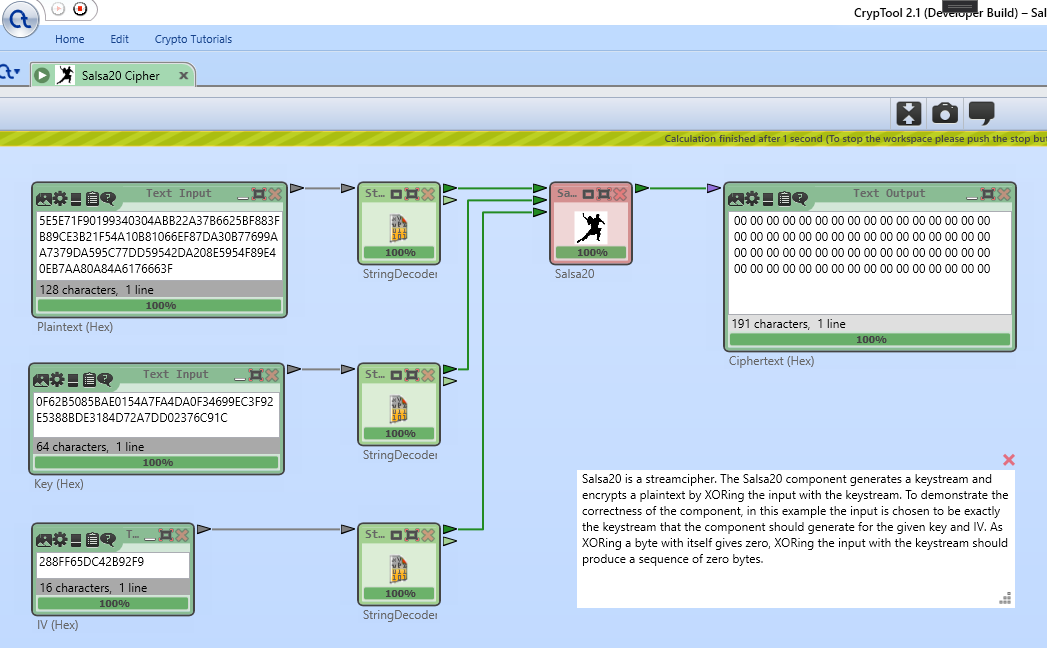
\includegraphics[width=\textwidth]{figures/ct2/salsa-crop.png}
\end{figure}

CrypTool 2 already has a plugin for the Salsa20 cipher but without a visualization.

During my work on the ChaCha visualization, I thought about how I could reuse my code for the ChaCha visualization to create a visualization for the Salsa20 cipher. I figured that it would not be as straight-forward as I assumed in the beginning since the visualization goes very into detail and thus the differences would involve at least different XAML code. For example, since the state is built up differently, the visualization about the state matrix initialization would need to be adapted. Also, the quarterround is slightly different which also needs to be reflected in the visualization. 

Nonetheless, I think that most of the codebase used for the ChaCha cipher could be reused to create a Salsa20 visualization, especially the navigation system and how the intermediate results are stored and retrieved for visualization. I will further discuss this in Chapter \ref{chap:futureWork}.


%%%%%%%%%%%%%%%%%%%%%%%%%%%%%%%%%%%%%%%%%%%%%%%%%%%%%%%%%%%%%%%%%%%%%%%%
\section{Other CrypTool 2 Cipher Visualizations}
\label{sec:otherCT2CipherVisualizations}

In this section, I will discuss ideas that I got from existing CrypTool 2 cipher visualizations which were also created by students during their bachelor thesis.

\subsection{AES Visualization}
\label{sec:aesVisualization}

\begin{figure}
\caption{AES visualization plugin}
\label{fig:aes}
\centering
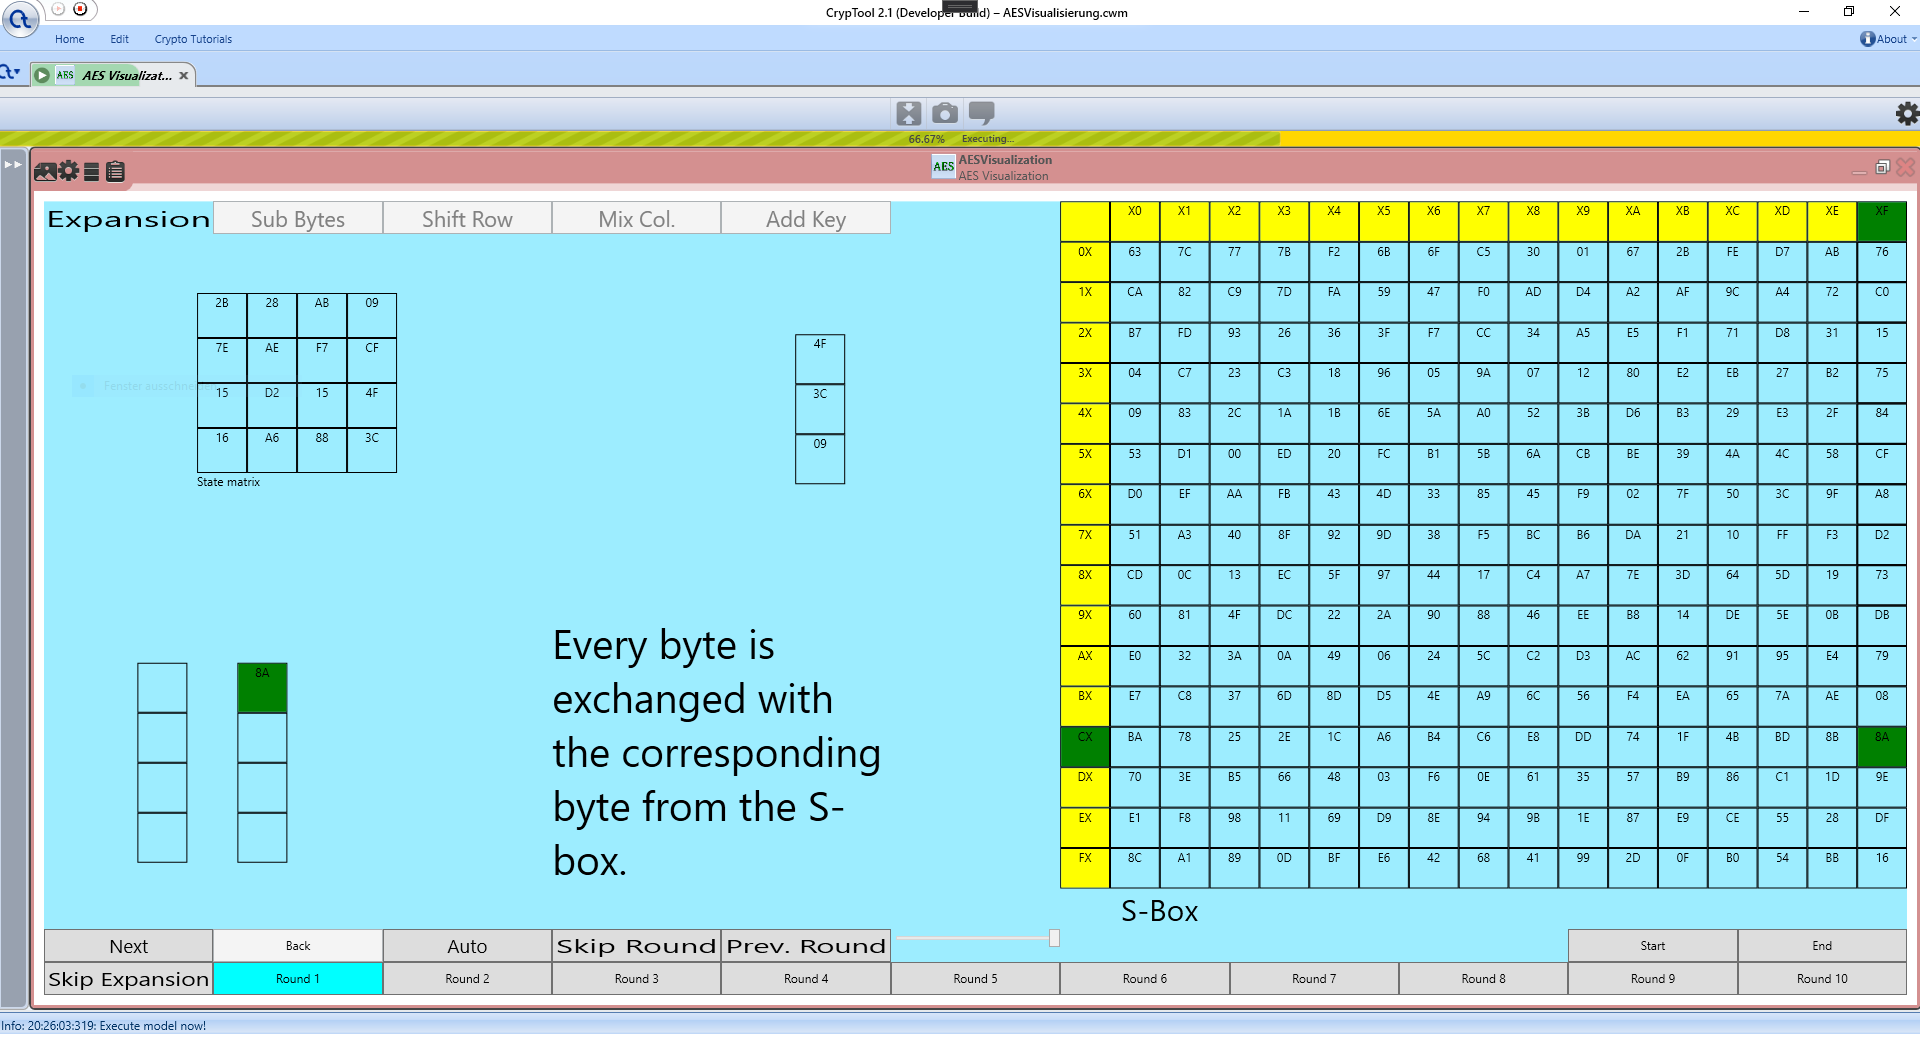
\includegraphics[width=\textwidth]{figures/ct2/aes.png}
\end{figure}

Matthias Becher created a visualization for the AES cipher during his bachelor thesis in 2016. It was the visualization of which I took the most inspiration for my own implementation. I also read through his bachelor thesis to see how he solved some of the problems that I encountered. For example, he wrote the following:

``The first big decision that had to be made was whether the states after each encryption operation would be calculated during the visualization or precalculated and stored at the start of the execution. One feature the plugin should have was to not only jump ahead to later operations but also to go back to previous ones. That means if the values were calculated during the visualization every time you went back they would have to be recalculated from the start. Therefore, I decided to precompute and store results of each operation in an array of byte arrays..'' \cite{aesthesis}

I came to the exact same conclusion that the values need to be precalculated for the reasons he mentioned.

Looking through his visualization, I liked how he changed the background of the elements to catch the user's attention. This is shown in Figure \ref{fig:aes}. I have used a similar mechanic during the ChaCha hash function visualization where I put a light blue background onto the state elements which will be used as the quarterround input. Also during the quarterround, I extensively used background coloring to tell the user where he should pay his attention.

Another thing I adopted from his visualization was the navigation in the top-left corner. I placed my page navigation there.

What I wanted to do differently in my navigation was to not show so many buttons all the time to the user. I was quite overwhelmed by all the buttons in the bottom navigation bar on the start even though they were disabled. Therefore, on pages which have no actions, I had no buttons in the bottom row. On pages with actions, a simple slider with a previous and next button did suffice. For the ChaCha hash function, which needed additional navigation, my navigation bar looked similar but still felt in my opinion less crowded, especially because I did not use buttons for every single round but a text input .

Further, I was confused why I could not use the ``Back'' button during the ``Expansion'' or ``Encryption'' step. For my plugin, I wanted to let the user navigate to any step in the visualization fairly simple. To achieve this, I needed to make sure that the user even knows where he is and where he needs to click to go to a particular step. To give the user the information he needed, I used the dedicated page navigation in the top-left corner which stays the same on every page and tells the user on which page he currently is using bold font. Further, I numbered every single action on each page together with an action text input and how many actions a page has. The text input enables the feature that I mentioned to let the user navigate to any step in the visualization fairly simple.

\subsection{DES Visualization}
\label{sec:desVisualization}

\begin{figure}
\caption{DES visualization plugin}
\label{fig:des}
\centering
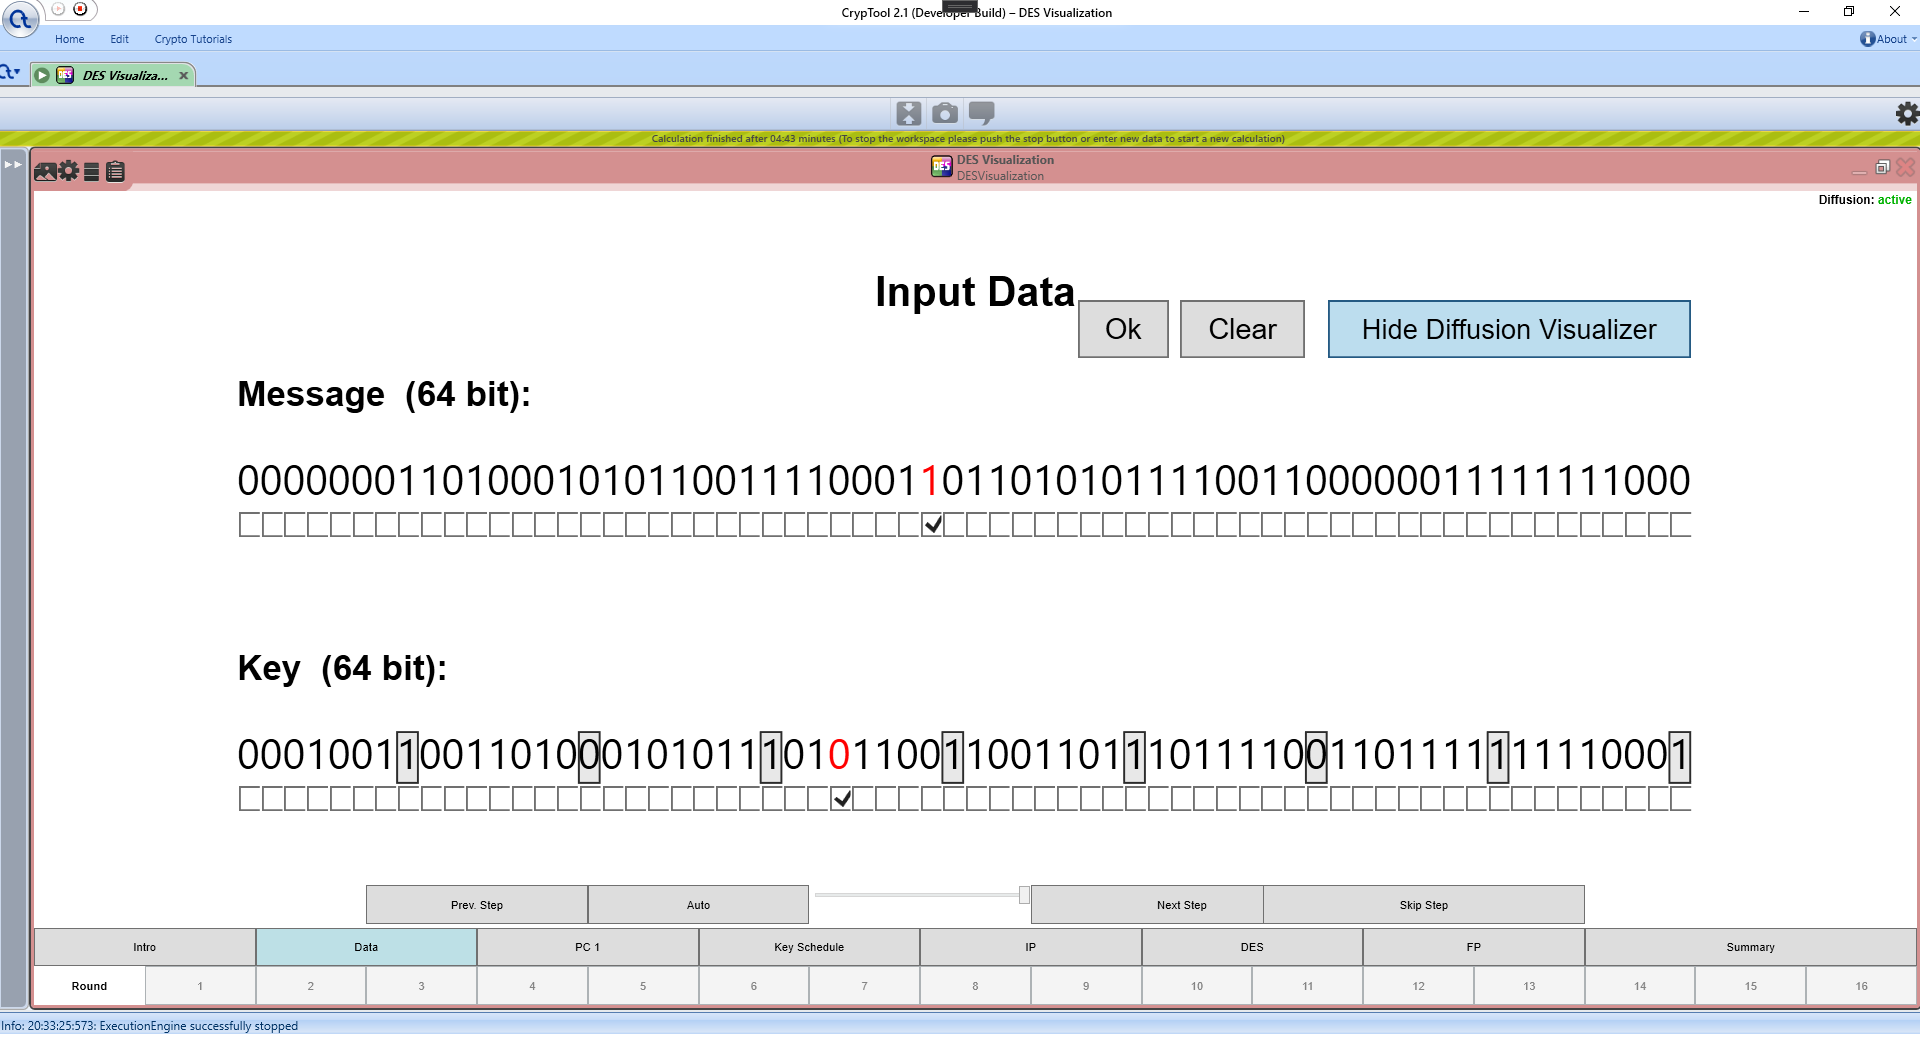
\includegraphics[width=\textwidth]{figures/ct2/des.png}
\end{figure}

\subsection{Avalanche Visualization}
\label{sec:avalancheVisualization}


